\documentclass[border=0pt]{standalone}
\usepackage{graphicx}
\usepackage{fancyvrb}
\usepackage{xcolor}
\usepackage{bm}
\usepackage{pgf}
\usepackage{tikz}
\usetikzlibrary{arrows,automata,positioning}


\definecolor{myGray}{rgb}{0.85,0.85,0.85}

\begin{document}

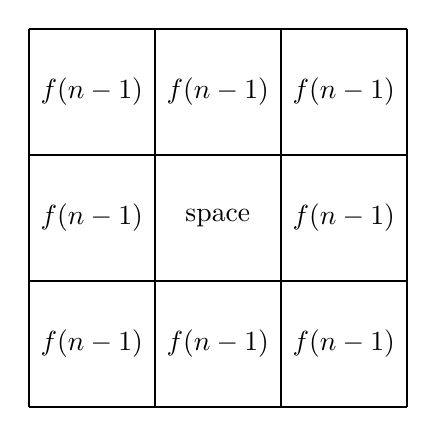
\begin{tikzpicture}[scale=0.8]
  \draw [step=2,thick] (0,0) grid (6,6);
  \node at (1,1) {$f(n-1)$};
  \node at (3,1) {$f(n-1)$};
  \node at (5,1) {$f(n-1)$};
  \node at (1,3) {$f(n-1)$};
  \node at (3,3) {space};
  \node at (5,3) {$f(n-1)$};
  \node at (1,5) {$f(n-1)$};
  \node at (3,5) {$f(n-1)$};
  \node at (5,5) {$f(n-1)$};
\end{tikzpicture}

\end{document}
